% CHAPTER 1

\begin{fullwidth}
\chapter{Introduction to Mountain Rescue \label{ch:chapter1}}
\end{fullwidth}
\minitoc
\thispagestyle{plain}
\renewcommand{\headrulewidth}{0.1pt}

Many people in the last few year have re-discovered a passion for winter mountain sports. Some of them have decided to explore the extreme version of this sports, like winter climbing or free-riding.

The increasing number of riders in extreme snow condition facilitates avalanches falling. Mountain Rescue Team is often called for search probable buried hikers, constrained to operate in an environment with an high residual risk. To facilitate the research, national and regional laws\cite{ARTVAobbligationLaw} have imposed the use of ARTVA transmitter, also called \emph{Avalanche Beacons}, for rider of non-equipped trails.

\section{Some statistics about the avalanche accidents}

During the year 2000, alpine countries decided to start an on line Database of avalanche victims, with the participation of the Italian council called \emph{A.I.NE.VA.}\marginnote{A.I.NE.VA: from the Italian \emph{Associazione Interregionale NEve e VAlanghe}}. The statistics show a mean of 18 victims per year in Italy. The number of accident is clearly related to the higher number of avalanche phenomena, strongly associated to the rising number of riders that are using snowboard. 

A deeper analysis of the data shows that the 40\% of the accidents have victims. Also, the number of buried was analyzed. Statistically:
\begin{itemize}
\item 60\% of the accidents have only one buried 
\item 34\% of the accidents have two or three buried 
\item 16\% of the accidents have four or more or more buried
\end{itemize}
\begin{marginfigure}
	\centering
	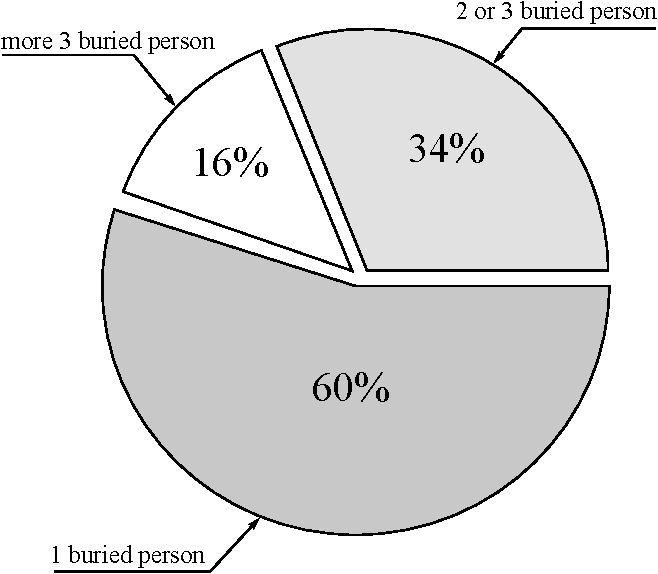
\includegraphics[width=5cm]{ch1/img/statistiche_sepolti.pdf}
	\caption{Number of buried}
\end{marginfigure}

Another important factor is the position of the overwhelms hikers:
\begin{itemize}
\item 37\% remain on the surface of the avalanche
\item 28\% are only partially buried
\item 35\% are completely buried
\end{itemize}

The survival curve, because of frostbite and hypothermia, without considerable traumas, has an upper limit of 15--18 minutes. Here is the the companion rescue that makes the real difference\cite{ManualeSciAlpinismo}.

One last important statistic is the number of hikers found with the ARTVA\marginnote{ARTVA: from the Italian \emph{Apparecchio Ricerca Travolti VAlanga}}. Considering the fact that the statistics do not take into account the episode of auto-rescue, the 7\% of the buried are found by the use of the receivers, a very small amount of the total. This data should be revised in the light of the advent of new digital ARTVA receivers, that simplify the searching method, and reduce the searching time \citep{hereforddigital}. 

As reported in \citep{Brugger2007}, within Europe and North America, avalanche airbags and avalanche transceiver reduce mortality, and companion rescue reduces incredibly the median duration of burial, remarking the extreme importance of those device for all mountaineers.

It is also known that 95\% of complete burial are in the layer between \num{-3} and\num{0} \si{\meter} of the avalanche.

\section{Avalanche Beacons}

There are two main typologies of avalanche transceiver. Differences are mostly in the user interface during receiving. We can divide in \emph{analog} and \emph{digital} ARTVA. Both device are equal for what concerns transmission. ARTVA can not be at the same time in transmission mode and receiving mode. Some models switch from receiving to transmission status after a scheduled amount of time. 

\subsection{Transmission Mode}

During transmission, beacons transmit a so-called \emph{wild-life tag}, or more simply, an intermittent signal at defined frequency, as stated in normative\cite{NormativaARVA}. From the normative, it is possible to extract more informations about the transmitted signal, that are listed in section \ref{sec:a1asegnale}.

\subsection{Receiving Mode}

The normative states for receiver:
\begin{itemize}
	\item the $(S+N)/N$ ratio of \num{6}\si{\decibel} at the terminal of electro--acoustic transducer
	\item a clear optical indication of direction for beacon with optical signal indication of direction
\end{itemize}
\marginnote{The Italian authority in Mountain Rescue is \emph{Soccorso Alpino e Speleologico Italiano}}

\myparagraph{Analog Beacons}
The analog beacon uses a cascade of filters and an identification circuit to extract the strength information of received signal. The strength is thus used as gain command for a sound generator, that rescuer uses to identify the direction of arrival. Typically, those ARTVA have a volume knob to perform a fine search. The main drawback is the extreme difficulty to perform a fast search, that requires an experienced user. Quoting \citep{457andfuture}: \emph{a better term for analog beacon would be \textbf{audible--based}}

\myparagraph{Digital Beacons}
Those beacons implements an user interface that indicates \emph{the field line direction and an artificial distance to the center of the field}. This simplicity makes those beacons perfect for unexperienced user and auto-rescue: those device \textbf{are strongly advised by the Mountain Rescue for all hikers, experienced or not}.

\begin{marginfigure}
	\centering
	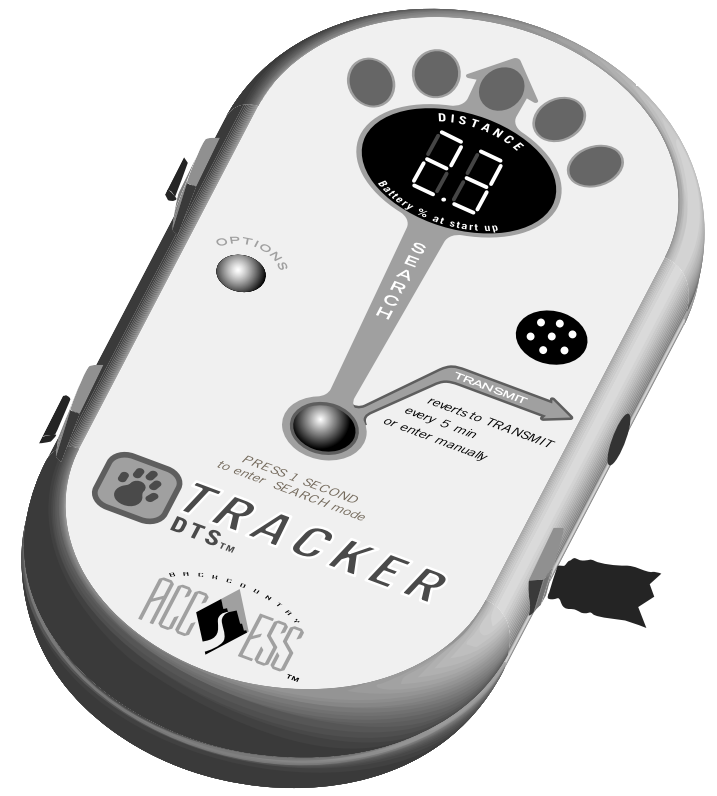
\includegraphics[width=4cm]{ch1/img/digital_baecon}
	\caption{Tracker DTS Avalanche Transceiver, a digital beacon}
\end{marginfigure}

Must be noted that the algorithm inside those transceivers runs on a very low power DPS, due to energy harvesting requirements, so often the rescuer must slow down his speed to gave time to the beacon to analyze received data. Also, it was pointed out from manufacturers that advanced techniques, like multi-buried identification and buried status (hearth-beat) make use of frequencies different from the one described in normative.

\subsection{Italian Mountain Rescue Intervention}
What happens after an avalanche? We interviewed some of the professionals of the Mountain Rescue Team in province of Trento, and asked them to explain us the actual procedure.

\myparagraph{Intervention on Avalanche}
The intervention begin after a witness call. Usually the witness is one of the hikers that is on the accident location. In the best situation, the witness begins the companion rescue procedure, with his own avalanche beacon, and calls the emergency number.

During the emergency call, the operator tries to understand the location, alerts the rescue team on shift and tries to figure out the general situation that the team may encounter. A rescue unit is formed by:
\begin{itemize}
\item Mountain Rescue heli-ambulance expert
\item Mountain Rescue canine unit
\item Health equip and nurse
\end{itemize}
If heli-ambulance is cleared to take off, those are the first rescuers on the avalanche. The clearance is related to weather and light conditions, because flight is performed by eye-sight. If heli-ambulance mission is aborted, Mountain Rescue team have to reach the avalanche with ground vehicle.

Under certain strict condition, it is possible to perform an ARTVA search from the helicopter.

Once arrived on the location, if residual risk make it possible, the rescue team is dropped from the heli-ambulance and starts the searching procedure, with canine unit and with personal ARTVAs. The rescuers with the beacons follow a scheme that allow them to cover the avalanche front. This scheme is called primary search. While a signal is identified, the rescuer start a fine search to pinpoint the buried position.

\myparagraph{Equipment}
There is a procedural and moral obligation in having the last generation device, even if does not exist a directive that defines a specific model for the equipment. Each rescuer has a VHF transmitter and cellphone, along with the personal beacon. 

It is possible to perform a search with other technology, like RECCO\sidenote[]{RECCO is a passive searching method, composed by a reflector included in hikers clothing, and a detector used by rescue teams. A RECCO detector usually performs passive search and \num{457}\si{\kilo\hertz} avalanche beacons search at the same time. The last generation detector has an average weight of \num{1}\si{\kilogram}, while the reflector weights only few grams. RECCO cannot be used for companion rescue}, even if the detector is heavy and not always reliable.

\section{State of the Art}

In this section we will analyze the state of the art in the field of beacons construction and signal analysis.

\subsection{Transmission}

Normative states the use of a very long wavelength ($\lunghezzaonda$) (\num{656}\si{\meter}). Such a long wavelength reduces the interference effects of snow, body and rocks and also multi-bouncing and multi-path effects\citep{balanis2012antenna} that may afflict some shorter waves. This is one of the main reason why GPS technology never erupted in this field\citep{457andfuture}.

This advantage also bring a consistent number of drawbacks, such as the fact that the search is always performed in near--field (distance less of $\lunghezzaonda/2\pi$). In the near--field, as we will see, interpretation of flux lines is quite complex, and it is difficult to derive a general direction of arrival algorithm.

Avalanche transceiver for companion rescue has to be small, therefore antennas and batteries has to be small. As we will see in the next chapter, to increase receiver antenna gain (also called effective height $\altezzaeffettiva$), ferrite core antennas are commonly used, but the efficiency and the noise introduced is not good. Those brings to transmitter that may be identified in the range of \numrange{40}{60}\si{\meter}, in function of type of receiver.

There is no big evolution in transmitters; almost all devices implement a simple amplitude--shifting--key (ASK) transmitter, build with an oscillator for the carrier, and a variable gain amplifier that modulates the intelligence signal.

\subsection{Reception}

Usually, an analog receiver has a little more bigger receiving radius with respect to a digital one. This difference is due to stronger filtration routines implemented in digital ARTVA, with respect to analog, and because of the dimension of the z--axis antenna.

A digital ARTVA implements multiple antennas. Some typical configurations are:
\begin{itemize}
\item two crossing antennas
\item three perpendicular antennas
\end{itemize}
The signal from whips are preprocessed using analog circuitry and then converted and processed in a DSP microprocessor. There are some advanced techniques\citep{Salos2007} implemented for the identification of the direction of the vectorial H--field, and also to help hikers and rescuers to find a transmitter. 

In general, the circuit may be resumed as follows:

\begin{figure}
	\centering
	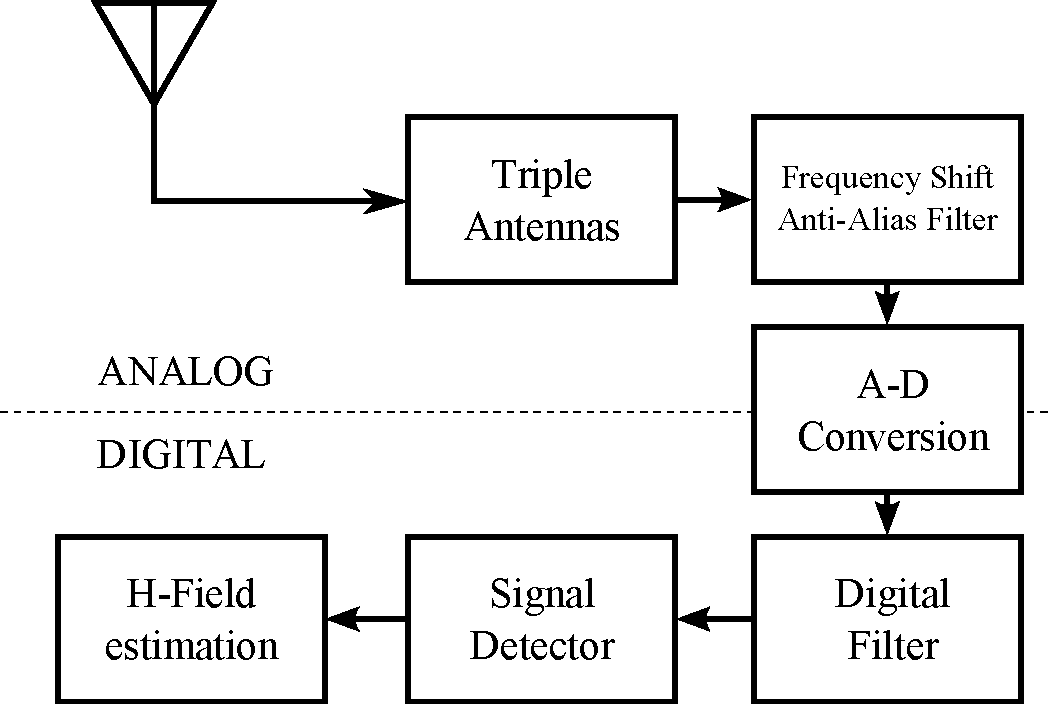
\includegraphics[width=7cm]{ch1/img/img_schema_arva.pdf}
	\caption{Block diagram of a commercial digital beacon, taken from \citep{Salos2007}}
	%\forceversofloat
\end{figure}


\begin{itemize}
\item signal is received through the antennas
\item the first stage of filtering is a frequency shift and  an anti-aliasing filter, that is necessary to avoid problems during AD-conversion
\item the signal is converted in the digital domain
\item other filtration techniques are analyzed  in \citep{Salos2007}, and are one of the main research topic in this field, in association with phase analysis to better understand the direction of the single components of the H--field
\item the signal detector and magnetic field estimator is implemented via software
\end{itemize}

One of the main challenge is the problem of the noise introduced by antennas. This noise is proportional to the received signal, phenomenon that induces an unsurmountable issue in the identification of multiple burial signal.

\subsection{Searching Algorithms}

\myparagraph{The magnetic momentum problem}
The main problem is the searching of the burial. Until now, only few are the example of automatic searching, while quite consolidated is the practice of the manual searching. One of the key aspects is the problem of the orientation of the transmitter: as we will see in the next chapter, the direction of the transmitter antenna change radically the shape of the field. From a general point of view, with respect to classical far--field identification problem, in this case we have to identify 6 state for each transmitter\sidenote[]{3 states refer to the position of the transmitter, while the latter 3 refers to the magnetic dipole momentum that is parallel to the axis of the antenna}, instead of 3, while we can only collect 3 measurements (the H--field vector components).

Even if there are some solutions for near--field qualitative direction of arrival, as explained in detail in \citep{hutchinson2000arrl}, typically those algorithms require a very prohibitive electro--mechanical circuitry, not suitable as mountain equipment (or in our case, a drone).

So far, only one solution earns the right to be cited: the solution proposed in \citep{pinies2006fast,pinies2006localization}, based upon Bayesian estimation theory and Kalman filters, is a remarkable attempt to find new approach to this problem, even if based on the weak assumption of a perfect knowledge of the covariance matrix related to the noise. One step ahead in this direction should be the redefinition of the problem in a dual form, from the Kalman filter to the information filter, in which the complete uncertainty is presented with a null matrix of the canonical form, instead of a infinite--valued matrix of the normal form. 

\myparagraph{Multiple Burial}
Those algorithms do not analyze the problem of multiple burial, and the subsequent possible situation of overlapping signal. An almost complete dissertation about this problem, with some test on beacon present on the market, may be found in \citep{signaloverlappingARVA1,signaloverlappingARVA2}. From those technical documents, distributed by one of the most well-know company in snow--safety, rises the evident lack of a solution for the overlapping problem, due to transmitted signal limitation. The most suggest solution is to run--away from an identified source in the hope to find another new signal. Some producer try to avoid this using parallel carrier frequency with additional information coded into intelligence signal (unique ID, heartbeat status, \dots). Those alternative frequencies are device/model dependent.

\myparagraph{A complex procedure}
Standard de facto is an algorithm of flux line following, in parallel with different assumption that user shall analyze, to derive the possible orientation of the buried person transmitting antenna, and subsequently find the best way to reach the hikers position. The complete explanation for the searching procedure is long even if not too complex, but based upon qualitative observation and deduction derived from expertise of the rescuer.

Generally speaking, what we need to know is the fact that a simple translation of this procedure in a machine with limited computational power is not practically possible.

A comprehensive description of the companion search and Mountain Rescue procedure could be found in \citep{ManualeSciAlpinismo}.

\section{Autonomous VTOL for buried searching}

The thesis is built around the main thread of inspect and derive the avionics of an autonomous VTOL. Even if avionics refer to the complete set of instrumentation and algorithms necessary to stabilize and control the flight, in this work we will focus on some of the main aspects necessary to perform the main task of buried searching.

This work is not the first attempt to bring an automatic drone on avalanches. Some remarkable examples are 
\begin{itemize}
\item SHERPA, European project born to create a robotic framework of helpers for Mountain Rescue, coordinated by University of Bologna
\item An user--piloted quad-copter research is just started in Politecnico di Torino
\item the project Alcedo from the Eidgen\"{o}ssische Technische Hochschule Z\"{u}rich\cite{projectAlcedoZurigo}
\end{itemize}

\subsection{Why the use of a VTOL?}
The use of a drone in the searching area depends on various factors. During design it is necessary to understand and think a system the fit entirely the actual search strategy.

One practical example of use could be a situation of high residual danger and an uncertainty about the presence of buried under the avalanche. In a case like that, the VTOL could be used to test the necessity of drop the rescue team on the avalanche.

The main advantage is obviously the ability to move faster on the avalanche with respect to an human rescuer, avoiding ground difficulties. At the same time, the drone should be able to identify and avoid obstacle like trees and ski--lift pillars.

\subsection{Quality Function Deployment}
The best way to define the characteristics of a new product is to inspect customer needs, and from qualitative user domain extrapolate quantitative engineering dimensions\cite{akao1994development}.

\myparagraph{Customer Needs}
From our interviews of Mountain Rescue members, we have derived some conclusions:
\begin{itemize}
\item one of the main cause of an avalanche is the weather, that modifies snow characteristics; during one day multiple avalanches may fall, so it is fundamental to guarantee a long, even if discontinue, operative time
\item the VTOL should be portable, with limited size and weight, but at the same time ready to be used in a short amount of time
\item all design process should take in to account the extreme low temperature and the high altitude (lower air density)
\item ARTVA device on the drone has to be robust with respect to electromagnetic interferences (propeller engines, radio, \dots)
\item user interface is simple while complete
\item the marking of the victims shall be hardware, with the use of visible darts
\end{itemize}
\begin{margintable}
	\begin{center}
		\begin{tabular}{ p{3.7cm} p{0.7cm} }
			\hline \textbf{Customer Need} & \textbf{Rating} \\ \hline
			Identifies buried person & 5 \\
			Is autonomous & 5 \\
			Returns to rescuer position & 5 \\
			Searches for the signall & 5 \\
			Is fast & 5 \\
			Marks physically buried position & 5 \\
			Operates at avalanche temperatures & 5 \\
			Performs more than one operation during the day & 3 \\
			Is usable by anyone & 3 \\
			Is robust with respect to EM interferences & 5 \\
			Is portable in a \num{35}\si{\liter} bag & 3 \\
			Is quiet & 2 \\
			Is compatible with other rescue vehicles & 5 \\
			Disengages from the winch & 5 \\
			Respects ENAC normatives & 3 \\
			\hline
		\end{tabular}
	\end{center}
	\caption{Customer needs \label{tbl:customer_needs}}
\end{margintable}

We are now able to define a table \ref{tbl:customer_needs} in which at each customer needs a rating is given.

In future, the automatic recognition of the avalanche dimensions could be a good starting point for some advanced research in the field of computer vision, or the improvements of user interface using voice recognition over radio.

\myparagraph{Technical Specification}
The next step in the definition of a good design is a list of technical specifications that will help us to identify the most challenging problems in and the gravity of those problems with respect to the costumer needs.

For sure, one of the first and most challenging complication is the weight reduction, that guarantees a longer flying time. Also those elements are related to the number of  propulsion vector and the main dimension (the length of the arm). It is evident the correlation between the number of lift vectors with respect to the maximum wind interference.

For the definition of a good searching algorithm, as we will see, it is important a good resolution of position and attitude of the drone; while to avoid obstacle it is important the resolution and the maximum revealing distance of the range finders.

One final aspect that should be considered are the data related to the system that performs the marking of a buried person.

All the specifications are listed in table \ref{tbl:tech_specs}
\begin{margintable}
	\begin{center}
		\begin{tabular}{ p{3.7cm}  p{0.7cm} }
			\hline \textbf{Technical Spec.} & \textbf{Dim.}  \\ \hline
			Flying time & \si{\minute} \\
			Weight & \si{\kilogram} \\
			N. of antennas & ~ \\
			Battery Temperature & \si{\celsius} \\
			Range Ultrasonic RF & \si{\meter} \\
			Arm Length & \si{\meter} \\
			Control TX distance & \si{\meter} \\
			GPS Resolution & \si{\meter} \\
			Lateral Speed & \si{\meter\per\second} \\
			 Wind Speed & \si{\meter\per\second} \\
			 ARTVA RX distance & \si{\meter} \\
			 Resolution Ultrasonic RF & \si{\meter} \\
			 Lift Force & \si{\newton} \\
			 N. dissembled pieces & ~ \\
			 N. Darts & ~ \\
			 N. Lift Vector & ~ \\
			 Maximum inclination & \si{\radian} \\
			 Operative height & \si{\meter} \\
			 IMU Resolution & \si{\meter\per\second} \\
			 Weight Marking Device & \si{\kilogram} \\
			 Weight Dart & \si{\kilogram} \\
			 Weight ARTVA & \si{\kilogram} \\
			\hline
		\end{tabular}
	\end{center}
	\caption{Technical specifications \label{tbl:tech_specs}}
\end{margintable}

% TODO invertire colonna 1 e 2 e nella nuoova colonna 2 inserire la dimensione 

\myparagraph{Merging the tables and comparison}
In table \ref{tbl:need_vs_spec} all data are compared with a weighting method. The table shows the comparison between technical specifications and customer needs and also between technical specifications and the other technical specifications.

\myparagraph{Components selection}
From the merged data it was possible to select the components that will be used in the prototype. All components are listed in table \ref{tbl:components_list}

We have also decide not to use a commercial ARTVA, but instead try to build a digital one from scratch. This will allow us to get a lighter model, and also extract exactly the information that we want from the received signal. Even if some device have a serial port, the output data are filtered with models that incorporate the possible speed of a rescue, that is different from our VTOL.
\begin{table}
	\begin{center}
		\begin{tabular}{ p{0.3cm} p{3.7cm} p{3.7cm} p{1cm} }
			\hline \scriptsize{\textbf{N}} & \footnotesize{\textbf{Component}} & \scriptsize{\textbf{Description}} & \footnotesize{\textbf{Price}} \\ \hline
			\scriptsize{$1\times$} & \footnotesize{Autoquad 6 Flight Controller} & \scriptsize{Imu board and stabilization controller} & \footnotesize{299.00\texteuro} \\
			\scriptsize{$6\times$} & \footnotesize{Autoquad ESC32} & \scriptsize{Electronic speed controller} & \footnotesize{239.40\texteuro} \\
			\scriptsize{$6\times$} & \footnotesize{Flyfuino HE4108 700kV Outrunner} & \scriptsize{Motors} & \footnotesize{299.40\texteuro} \\
			\scriptsize{$6\times$} & \footnotesize{HQ 12\inch per 4.5\inch CW and CCW Carbon propeller} & \scriptsize{Propeller} & \footnotesize{73.80\texteuro} \\
			\scriptsize{$2\times$} & \footnotesize{SLS Xtron \num{5000}\si{\milli\ampere\hour} \num{14.8}\si{\volt}} & \footnotesize{Batteries} & \footnotesize{119.98\texteuro} \\
			\scriptsize{$3\times$} & \footnotesize{USB UART Adapter} & \scriptsize{Bridge between USB and device UART} & \footnotesize{9.90\texteuro} \\
			\hline
			\multicolumn{3}{r}{\footnotesize{\textbf{Total}}}  & \footnotesize{1041.48\texteuro} \\
			\hline
		\end{tabular}
	\end{center}
	\caption{Components list \label{tbl:components_list}}
\end{table}

\newcommand{\rotatenovsmalll}[1]{\begin{sideways}\scriptsize{\textbf{#1}}\end{sideways}}
\newcommand{\smallbold}[1]{\scriptsize{\textbf{#1}}}

%\def\nine{\scriptsize{\textbf{9}}}
%\def\three{\scriptsize{3}}
\def\nine{\scriptsize{$\CIRCLE$}}
\def\three{\scriptsize{$\RIGHTcircle$}}
\def\point{\scriptsize{$\ocircle$}}

\def\upnin{\scriptsize{\begin{sideways}$\RHD$\end{sideways}}}
\def\upthr{\scriptsize{\begin{sideways}$\rhd$\end{sideways}}}
\def\dwnin{\scriptsize{\begin{sideways}$\LHD$\end{sideways}}}
\def\dwthr{\scriptsize{\begin{sideways}$\lhd$\end{sideways}}}

\begin{table*}[p]
    \centering
    \begin{tabular}{ b{4cm} b{0.08cm} b{0.08cm} b{0.08cm} b{0.08cm} b{0.08cm} b{0.08cm} b{0.08cm} b{0.08cm} b{0.08cm} b{0.08cm} b{0.08cm} b{0.08cm} b{0.08cm} b{0.08cm} b{0.08cm} b{0.08cm} b{0.08cm} b{0.08cm} b{0.08cm} b{0.08cm} b{0.08cm} b{0.08cm} }
    \hline
    \smallbold{Identifies buried person}                            &  \nine   &  \point  &  \nine   &  \point  &  \point  &  \point  &  \point  &  \nine   &  \three  &  \point  &  \nine   &  \point  &  \point  &  \point  &  \nine   &  \point  &  \point  &  \point  &  \point  &  \three  &  \three  &  \three  \\
    \smallbold{Is autonomous}                                       &  \three  &  \nine   &  \nine   &  \point  &  \nine   &  \point  &  \nine   &  \nine   &  \three  &  \nine   &  \nine   &  \three  &  \point  &  \point  &  \point  &  \point  &  \point  &  \point  &  \nine   &  \point  &  \point  &  \point  \\
    \smallbold{Returns to rescuers position}                        &  \nine   &  \point  &  \point  &  \point  &  \point  &  \point  &  \nine   &  \nine   &  \three  &  \nine   &  \point  &  \nine   &  \point  &  \point  &  \point  &  \point  &  \point  &  \three  &  \three  &  \point  &  \point  &  \point  \\
    \smallbold{Searches for the signal}                             &  \nine   &  \point  &  \nine   &  \point  &  \point  &  \point  &  \point  &  \nine   &  \nine   &  \point  &  \nine   &  \point  &  \point  &  \point  &  \point  &  \point  &  \point  &  \nine   &  \three  &  \point  &  \point  &  \nine   \\
    \smallbold{Is fast}                                             &  \three  &  \nine   &  \point  &  \point  &  \three  &  \nine   &  \point  &  \nine   &  \point  &  \nine   &  \point  &  \nine   &  \nine   &  \point  &  \point  &  \nine   &  \nine   &  \point  &  \nine   &  \three  &  \point  &  \point  \\
    \smallbold{Marks physically buried position}                    &  \point  &  \point  &  \point  &  \point  &  \point  &  \point  &  \nine   &  \nine   &  \point  &  \nine   &  \point  &  \nine   &  \point  &  \point  &  \nine   &  \point  &  \point  &  \point  &  \nine   &  \three  &  \nine   &  \point  \\
    \smallbold{Operates at avalanche temperature}                   &  \point  &  \point  &  \point  &  \nine   &  \point  &  \point  &  \nine   &  \nine   &  \point  &  \nine   &  \point  &  \nine   &  \point  &  \point  &  \point  &  \point  &  \point  &  \nine   &  \nine   &  \nine   &  \point  &  \point  \\
    \smallbold{Performs more than one operation during the day}     &  \nine   &  \three  &  \point  &  \nine   &  \point  &  \point  &  \point  &  \point  &  \point  &  \point  &  \point  &  \point  &  \three  &  \point  &  \three  &  \three  &  \point  &  \three  &  \point  &  \point  &  \three  &  \point  \\
    \smallbold{Is usable by anyone}                                 &  \point  &  \point  &  \point  &  \point  &  \three  &  \point  &  \three  &  \point  &  \point  &  \point  &  \point  &  \point  &  \point  &  \nine   &  \point  &  \point  &  \point  &  \point  &  \point  &  \three  &  \point  &  \point  \\
    \smallbold{Is robust with respect to EM}                        &  \point  &  \point  &  \nine   &  \point  &  \point  &  \point  &  \nine   &  \nine   &  \point  &  \nine   &  \three  &  \point  &  \point  &  \point  &  \point  &  \nine   &  \point  &  \point  &  \nine   &  \point  &  \point  &  \nine   \\
    \smallbold{Is portable  in a 35L bag}                           &  \point  &  \nine   &  \point  &  \three  &  \point  &  \nine   &  \point  &  \point  &  \point  &  \point  &  \point  &  \point  &  \point  &  \nine   &  \nine   &  \nine   &  \point  &  \point  &  \point  &  \point  &  \three  &  \nine   \\
    \smallbold{Is quiet}                                            &  \point  &  \point  &  \point  &  \point  &  \point  &  \point  &  \point  &  \point  &  \three  &  \point  &  \point  &  \point  &  \three  &  \point  &  \point  &  \nine   &  \three  &  \point  &  \point  &  \nine   &  \point  &  \point  \\
    \smallbold{Is compatible with other rescue vehicles}            &  \point  &  \point  &  \nine   &  \nine   &  \point  &  \point  &  \point  &  \nine   &  \point  &  \point  &  \nine   &  \point  &  \point  &  \point  &  \point  &  \point  &  \point  &  \point  &  \point  &  \point  &  \point  &  \point  \\
    \smallbold{Disengages from the winch}                           &  \point  &  \three  &  \point  &  \three  &  \point  &  \three  &  \point  &  \point  &  \point  &  \point  &  \point  &  \point  &  \point  &  \point  &  \point  &  \point  &  \point  &  \point  &  \point  &  \point  &  \nine   &  \nine   \\
    \smallbold{Respects ENAC normatives}                            &  \point  &  \nine   &  \three  &  \nine   &  \nine   &  \nine   &  \nine   &  \three  &  \three  &  \three  &  \point  &  \nine   &  \point  &  \point  &  \point  &  \nine   &  \point  &  \nine   &  \point  &  \three  &  \three  &  \three  \\
    \hline \\ 


    \scriptsize{\textbf{Legend}: \newline \scriptsize{\emph{Cust. needs vs. Tech. spec.}: \newline\point \hspace{1.5mm} no relation \newline\three \hspace{1.5mm} light relation \newline\nine \hspace{1.5mm} strong relation \newline \emph{Tech. spec. vs. Tech. spec.}: \newline\dwnin \hspace{1.5mm} negative strong relation \newline\dwthr \hspace{1.5mm} negative light relation \newline\point \hspace{1.5mm} no relation \newline\upthr \hspace{1.5mm} positive light relation \newline\upnin \hspace{1.5mm} positive strong relation}}

     & \rotatenovsmalll{Flying time} & \rotatenovsmalll{Weight} & \rotatenovsmalll{N. ARTVA antennas} & \rotatenovsmalll{Battery Temperature} & \rotatenovsmalll{Range Ultrasonic RF} & \rotatenovsmalll{Arm Length} & \rotatenovsmalll{Control TX distance} & \rotatenovsmalll{GPS resolution} & \rotatenovsmalll{Lateral speed} & \rotatenovsmalll{Wind speed} & \rotatenovsmalll{ARTVA RX distance} & \rotatenovsmalll{Resolution Ultrasonic RF} & \rotatenovsmalll{Lift Force} & \rotatenovsmalll{N. dissembled pieces} & \rotatenovsmalll{N. Darts} & \rotatenovsmalll{N. Lift vector} & \rotatenovsmalll{Maximum inclination} & \rotatenovsmalll{Operative Height} & \rotatenovsmalll{IMU resolution} & \rotatenovsmalll{Weight Marking Device} & \rotatenovsmalll{Weight Darts} & \rotatenovsmalll{Weight ARTVA}  \\
    \hline
    \multicolumn{2}{r}{\smallbold{Flying Time}}                                &  \dwnin  &  \dwthr  &  \dwthr  &  \point  &  \dwnin  &  \upthr  &  \upthr  &  \dwthr  &  \dwthr  &  \point  &  \point  &  \dwthr  &  \dwthr  &  \dwthr  &  \point  &  \point  &  \dwthr  &  \point  &  \dwnin  &  \dwnin  &  \dwnin  \\
    \multicolumn{3}{r}{\smallbold{Weight}}                                                &  \upnin  &  \upthr  &  \point  &  \upthr  &  \point  &  \point  &  \point  &  \upthr  &  \point  &  \point  &  \upthr  &  \upnin  &  \upnin  &  \upnin  &  \point  &  \point  &  \point  &  \upnin  &  \upnin  &  \upnin  \\
    \multicolumn{4}{r}{\smallbold{N. ARTVA antennas}}                                                &  \point  &  \point  &  \point  &  \point  &  \point  &  \point  &  \point  &  \upnin  &  \point  &  \dwthr  &  \upnin  &  \point  &  \point  &  \point  &  \point  &  \point  &  \point  &  \point  &  \upnin  \\
    \multicolumn{5}{r}{\smallbold{Battery temperature}}                                                         &  \point  &  \point  &  \point  &  \point  &  \dwthr  &  \point  &  \point  &  \point  &  \dwnin  &  \point  &  \point  &  \point  &  \point  &  \upnin  &  \point  &  \point  &  \point  &  \point  \\
    \multicolumn{6}{r}{\smallbold{Range Ultrasonic RF}}                                                                    &  \point  &  \point  &  \point  &  \upthr  &  \upthr  &  \point  &  \dwnin  &  \point  &  \point  &  \point  &  \point  &  \upnin  &  \point  &  \point  &  \point  &  \point  &  \point  \\
    \multicolumn{7}{r}{\smallbold{Arm length}}                                                                                        &  \point  &  \point  &  \upnin  &  \upnin  &  \point  &  \point  &  \dwthr  &  \point  &  \point  &  \point  &  \upthr  &  \point  &  \point  &  \point  &  \point  &  \point  \\
    \multicolumn{8}{r}{\smallbold{Control TX distance}}                                                                                          &  \upthr  &  \upthr  &  \point  &  \point  &  \point  &  \point  &  \point  &  \point  &  \point  &  \point  &  \point  &  \point  &  \point  &  \point  &  \point  \\
    \multicolumn{9}{r}{\smallbold{GPS Resolution}}                                                                                                          &  \point  &  \upthr  &  \point  &  \point  &  \point  &  \point  &  \point  &  \point  &  \point  &  \point  &  \dwthr  &  \point  &  \point  &  \point  \\
    \multicolumn{10}{r}{\smallbold{Lateral speed}}                                                                                                                     &  \point  &  \point  &  \point  &  \upnin  &  \point  &  \point  &  \upnin  &  \upnin  &  \point  &  \point  &  \point  &  \point  &  \point  \\
    \multicolumn{11}{r}{\smallbold{Wind speed}}                                                                                                                                   &  \point  &  \point  &  \upnin  &  \point  &  \point  &  \upnin  &  \upthr  &  \point  &  \upnin  &  \upthr  &  \upthr  &  \upthr  \\
    \multicolumn{12}{r}{\smallbold{ARTVA RX distance}}                                                                                                                                       &  \point  &  \point  &  \point  &  \point  &  \point  &  \point  &  \point  &  \point  &  \point  &  \point  &  \upnin  \\
    \multicolumn{13}{r}{\smallbold{Resolution Ultrasonic RF}}                                                                                                                                           &  \point  &  \point  &  \point  &  \point  &  \point  &  \point  &  \point  &  \point  &  \point  &  \point  \\
    \multicolumn{14}{r}{\smallbold{Lift Force}}                                                                                                                                                                    &  \point  &  \point  &  \upnin  &  \upthr  &  \upnin  &  \point  &  \point  &  \point  &  \point  \\
    \multicolumn{15}{r}{\smallbold{N. disassembled pieces}}                                                                                                                                                                   &  \upnin  &  \upnin  &  \point  &  \point  &  \point  &  \upthr  &  \upthr  &  \upthr  \\
    \multicolumn{16}{r}{\smallbold{N. Darts}}                                                                                                                                                                                            &  \point  &  \point  &  \point  &  \point  &  \upnin  &  \dwnin  &  \point  \\
    \multicolumn{17}{r}{\smallbold{N. Lift vector}}                                                                                                                                                                                                 &  \upnin  &  \upnin  &  \point  &  \point  &  \point  &  \point  \\
    \multicolumn{18}{r}{\smallbold{Maximum inclination}}                                                                                                                                                                                                       &  \dwthr  &  \point  &  \point  &  \point  &  \point  \\
    \multicolumn{19}{r}{\smallbold{Operative Height}}                                                                                                                                                                                                                     &  \point  &  \point  &  \point  &  \point  \\
    \multicolumn{20}{r}{\smallbold{IMU Resolution}}                                                                                                                                                                                                                                  &  \point  &  \point  &  \point  \\
    \multicolumn{21}{r}{\smallbold{Weight Marking Device}}                                                                                                                                                                                                                                      &  \upnin  &  \point  \\
    \multicolumn{22}{r}{\smallbold{Weight Darts}}                                                                                                                                                                                                                                                          &  \point  \\
    \end{tabular}
    \caption{Comparison Table\label{tbl:need_vs_spec}}
    \forceversofloat
\end{table*}

%\marginnote{\textbf{How to read table \ref{tbl:need_vs_spec}}: \newline \scriptsize{\emph{Cust. needs vs. Tech. spec.}: \newline\point \hspace{1.5mm} no relation \newline\three \hspace{1.5mm} light relation \newline\nine \hspace{1.5mm} strong relation \newline \emph{Tech. spec. vs. Tech. spec.}: \newline\dwnin \hspace{1.5mm} negative strong relation \newline\dwthr \hspace{1.5mm} negative light relation \newline\point \hspace{1.5mm} no relation \newline\upthr \hspace{1.5mm} positive light relation \newline\upnin \hspace{1.5mm} positive strong relation}}

\let\nine\undefined
\let\three\undefined
\let\point\undefined
\let\upnin\undefined
\let\upthr\undefined
\let\dwthr\undefined
\let\dwnin\undefined

\FloatBarrier
